\documentclass{article}

\usepackage{graphicx}
\usepackage{subcaption}
\usepackage{pgffor}
\usepackage{amsmath, amsthm, amssymb, amsfonts}
\usepackage{thmtools}
\usepackage{graphicx}
\usepackage{setspace}
\usepackage{geometry}
\usepackage{float}
\usepackage{hyperref}
\usepackage[utf8]{inputenc}
\usepackage[english]{babel}
\usepackage{framed}
\usepackage[dvipsnames]{xcolor}
\usepackage{tcolorbox}

\colorlet{LightGray}{White!90!Periwinkle}
\colorlet{LightOrange}{Orange!15}
\colorlet{LightGreen}{Green!15}

\newcommand{\HRule}[1]{\rule{\linewidth}{#1}}

\declaretheoremstyle[name=Theorem,]{thmsty}
\declaretheorem[style=thmsty,numberwithin=section]{theorem}
\tcolorboxenvironment{theorem}{colback=LightGray}

\declaretheoremstyle[name=Proposition,]{prosty}
\declaretheorem[style=prosty,numberlike=theorem]{proposition}
\tcolorboxenvironment{proposition}{colback=LightOrange}

\declaretheoremstyle[name=Principle,]{prcpsty}
\declaretheorem[style=prcpsty,numberlike=theorem]{principle}
\tcolorboxenvironment{principle}{colback=LightGreen}

\setstretch{1.2}
\geometry{
    textheight=9in,
    textwidth=5.5in,
    top=1in,
    headheight=12pt,
    headsep=25pt,
    footskip=30pt
}

% ------------------------------------------------------------------------------

\begin{document}

% ------------------------------------------------------------------------------
% Cover Page and ToC
% ------------------------------------------------------------------------------

\title{ \normalsize \textsc{}
		\\ [2.0cm]
		\HRule{1.5pt} \\
		\LARGE \textbf{\uppercase{CS 460: INTRO TO COMPUTATIONAL ROBOTICS}
		\HRule{2.0pt} \\ [0.6cm] \LARGE{Assignment 1} \vspace*{10\baselineskip}}
		}
\date{}
\author{\textbf{Andy Xu} \\ axx2@rutgers.edu \\
    \textbf{Tasha Pais} \\ tdp74@rutgers.edu \\
		Rutgers University, Department of Computer Science \\
		October 8, 2023}


\maketitle
\newpage

\section{Generate, Visualize and Store 2D Polygonal Scenes}

\section*{Examples and Configurations}
The first 4 scenes were generated with the following configuration:
\begin{itemize}
    \item 3 min vertices
    \item 8 max vertices
    \item 0.05 min radius
    \item 0.3 max radius
\end{itemize}
The setting that they differed in was the number of polygons. Scene 1 has 5, Scene 2 has 8, Scene 3 has 16, and Scene 4 has 32.
\section*{Approach}
The approach followed the strategy mentioned in the assignment.
The program generates a convex polygon by first determining the number of vertices within a given range.
Then, it generates random angles (in radians) and radii for each vertex.
Using these angles and radii, it calculates the x and y coordinates of each vertex and stores them in the vertices array.
The ConvexHull function from scipy.spatial is used to compute the convex hull of the generated vertices, ensuring the resulting polygon is convex.

\foreach \scene in {1,2,3,4,5} {
    \begin{figure}[H]
        \centering
        \includegraphics[width=0.7\linewidth]{robotics-project1/scene\scene.png}
        \caption{Scene \scene}
        \label{fig:scene_\scene_}
    \end{figure}
}

\section{2D Collision Checking for Convex Polygons}
\section*{Approach}
The approach followed the mentioned strategy in the assignment.
The program first checks all pairs of line segments between polygons for collisions.
It then checks if any of the vertices are inside another polygon using a ray casting algorithm.
This handles the case where a polygon is completely inside another one.
Any polygons that are not marked as intersecting after these checks are plotted as unfilled. Otherwise, they are plotted as filled.
Below are the collision plots of the 5 figures from Part 1:

\foreach \scene in {1,2,3,4,5} {
    \begin{figure}[H]
        \centering
        \includegraphics[width=0.7\linewidth]{robotics-project1/collision_plot\scene.png}
        \caption{Collision Plot \scene}
        \label{fig:scene_\scene_}
    \end{figure}
}

\section{Collision-Free Navigation for a 2D Rigid Body}

The four keys used to control the rectangle on its own axes are:
\begin{itemize}
    \item 'w' for forward
    \item 'z' for backward
    \item 'a' for anticlockwise 
    \item 'd' for clockwise
\end{itemize}

\section*{Scenes with Different Orientations}

\title{Computing the Minkowski Sum in Scene Navigation}
\maketitle

\section*{Minkowski Sum: A Brief Overview}

The Minkowski sum is a mathematical operation that combines two shapes, \(P\) and \(Q\), to create a new shape, \(P \oplus Q\), that represents all possible translations of \(Q\) that maintains contact with \(P\) without penetrating it. When considering convex polygons, such as rectangles, and another polygon (either convex or non-convex), this operation can be described geometrically and algebraically.

\section*{Geometric Explanation}

Given two sets of points \(P = \{p_1, p_2, \ldots, p_n\}\) and \(Q = \{q_1, q_2, \ldots, q_m\}\), the Minkowski sum, denoted as \(P \oplus Q\), is computed as:

\[
P \oplus Q = \{p + q \,|\, p \in P, q \in Q\}
\]

This means that the Minkowski sum is formed by adding each point \(q\) in \(Q\) to each point \(p\) in \(P\), resulting in a new set of points that defines a new shape.

\section*{Algorithmic Explanation}

In the context of robot navigation within a scene containing obstacles:

\begin{enumerate}
    \item For each obstacle polygon in the scene, extract its vertices \(P\).
    \item Define a reference polygon \(Q\) (e.g., the robot shape, often a rectangle), extract its vertices, and possibly rotate it according to the desired orientation.
    \item Compute the Minkowski sum \(P \oplus Q\) by adding every vertex \(q \in Q\) to every vertex \(p \in P\). The result is a new set of vertices that define a new polygon.
    \item (Optional) To obtain a clean, non-intersecting polygon from the Minkowski sum, compute the convex hull of the resulting set of points.
    \item The resulting polygon represents the configuration space obstacle, a region that the reference point of \(Q\) must avoid to prevent collision with \(P\).
\end{enumerate}
% Iterate through scenes and orientations, adjusting numbers as needed.
\foreach \scene in {1,2,3,4,5} { 
    \foreach \orient in {1,2,3} {
        \begin{figure}[H]
            \centering
            \includegraphics[width=0.7\linewidth]{scene_\scene_orientation_\orient.png}
            \caption{Scene \scene, Orientation \orient}
            \label{fig:scene_\scene_\orient}
        \end{figure}
    }
}
\section{Collision-free Movement of a Planar Arm}

Initialized arms and obstacles:
\begin{figure}[h!]
    \centering
    \begin{subfigure}{0.45\textwidth}
        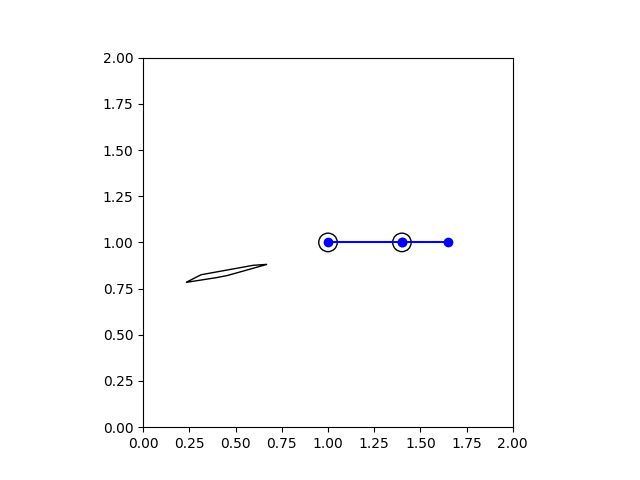
\includegraphics[width=\textwidth]{polygon_scene1.png}
        \caption{Scene 1}
    \end{subfigure}
    \hfill
    \begin{subfigure}{0.45\textwidth}
        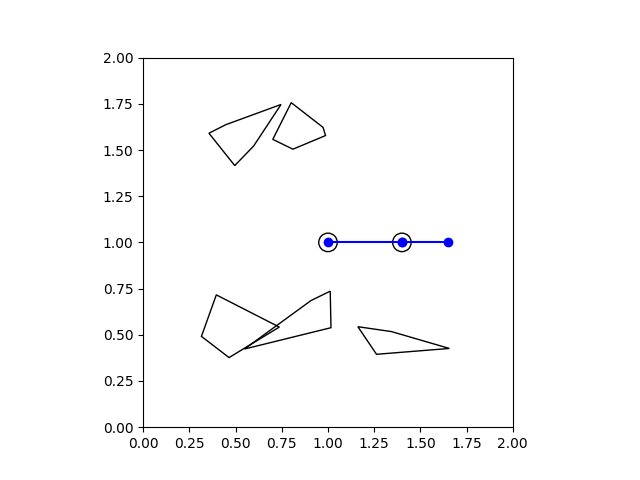
\includegraphics[width=\textwidth]{polygon_scene2.png}
        \caption{Scene 2}
    \end{subfigure}
    \\
    \begin{subfigure}{0.45\textwidth}
        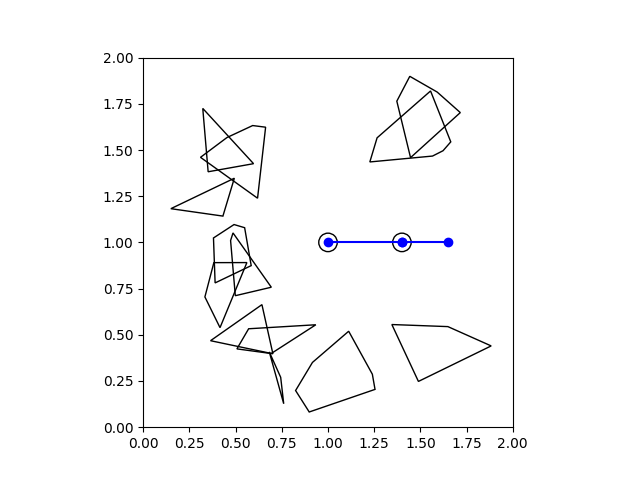
\includegraphics[width=\textwidth]{polygon_scene3.png}
        \caption{Scene 3}
    \end{subfigure}
    \hfill
    \begin{subfigure}{0.45\textwidth}
        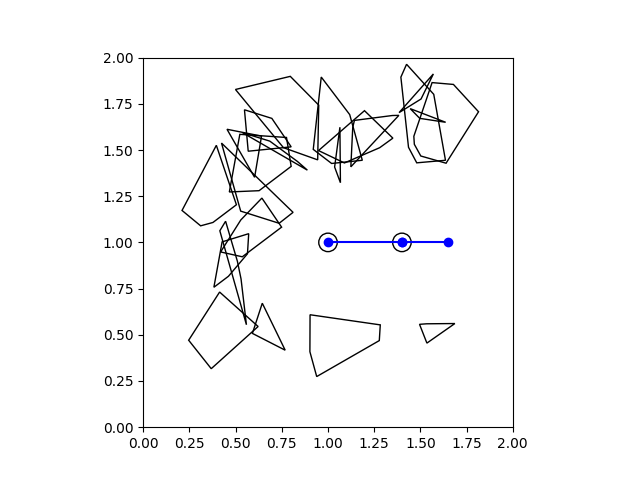
\includegraphics[width=\textwidth]{polygon_scene4.png}
        \caption{Scene 4}
    \end{subfigure}
    \\
    \begin{subfigure}{0.45\textwidth}
        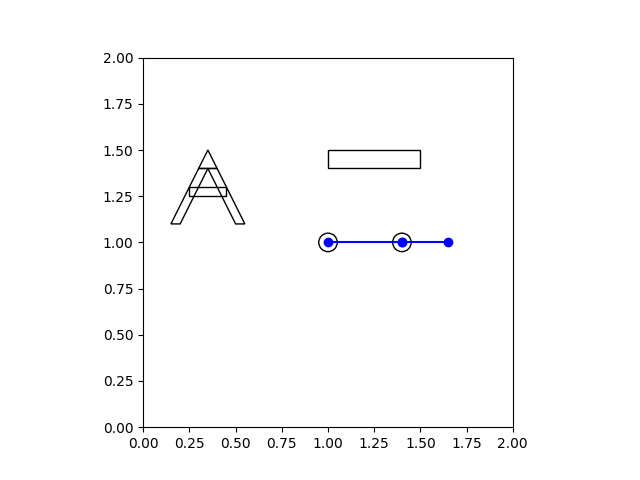
\includegraphics[width=\textwidth]{polygon_scene5.png}
        \caption{Scene 5}
    \end{subfigure}
    \caption{Polygonal scenes with a planar arm, showing different configurations.}
    \label{fig:scenes}
\end{figure}

Configuration spaces for planar arm:
\begin{figure}[h!]
    \centering
    \begin{subfigure}{0.45\textwidth}
        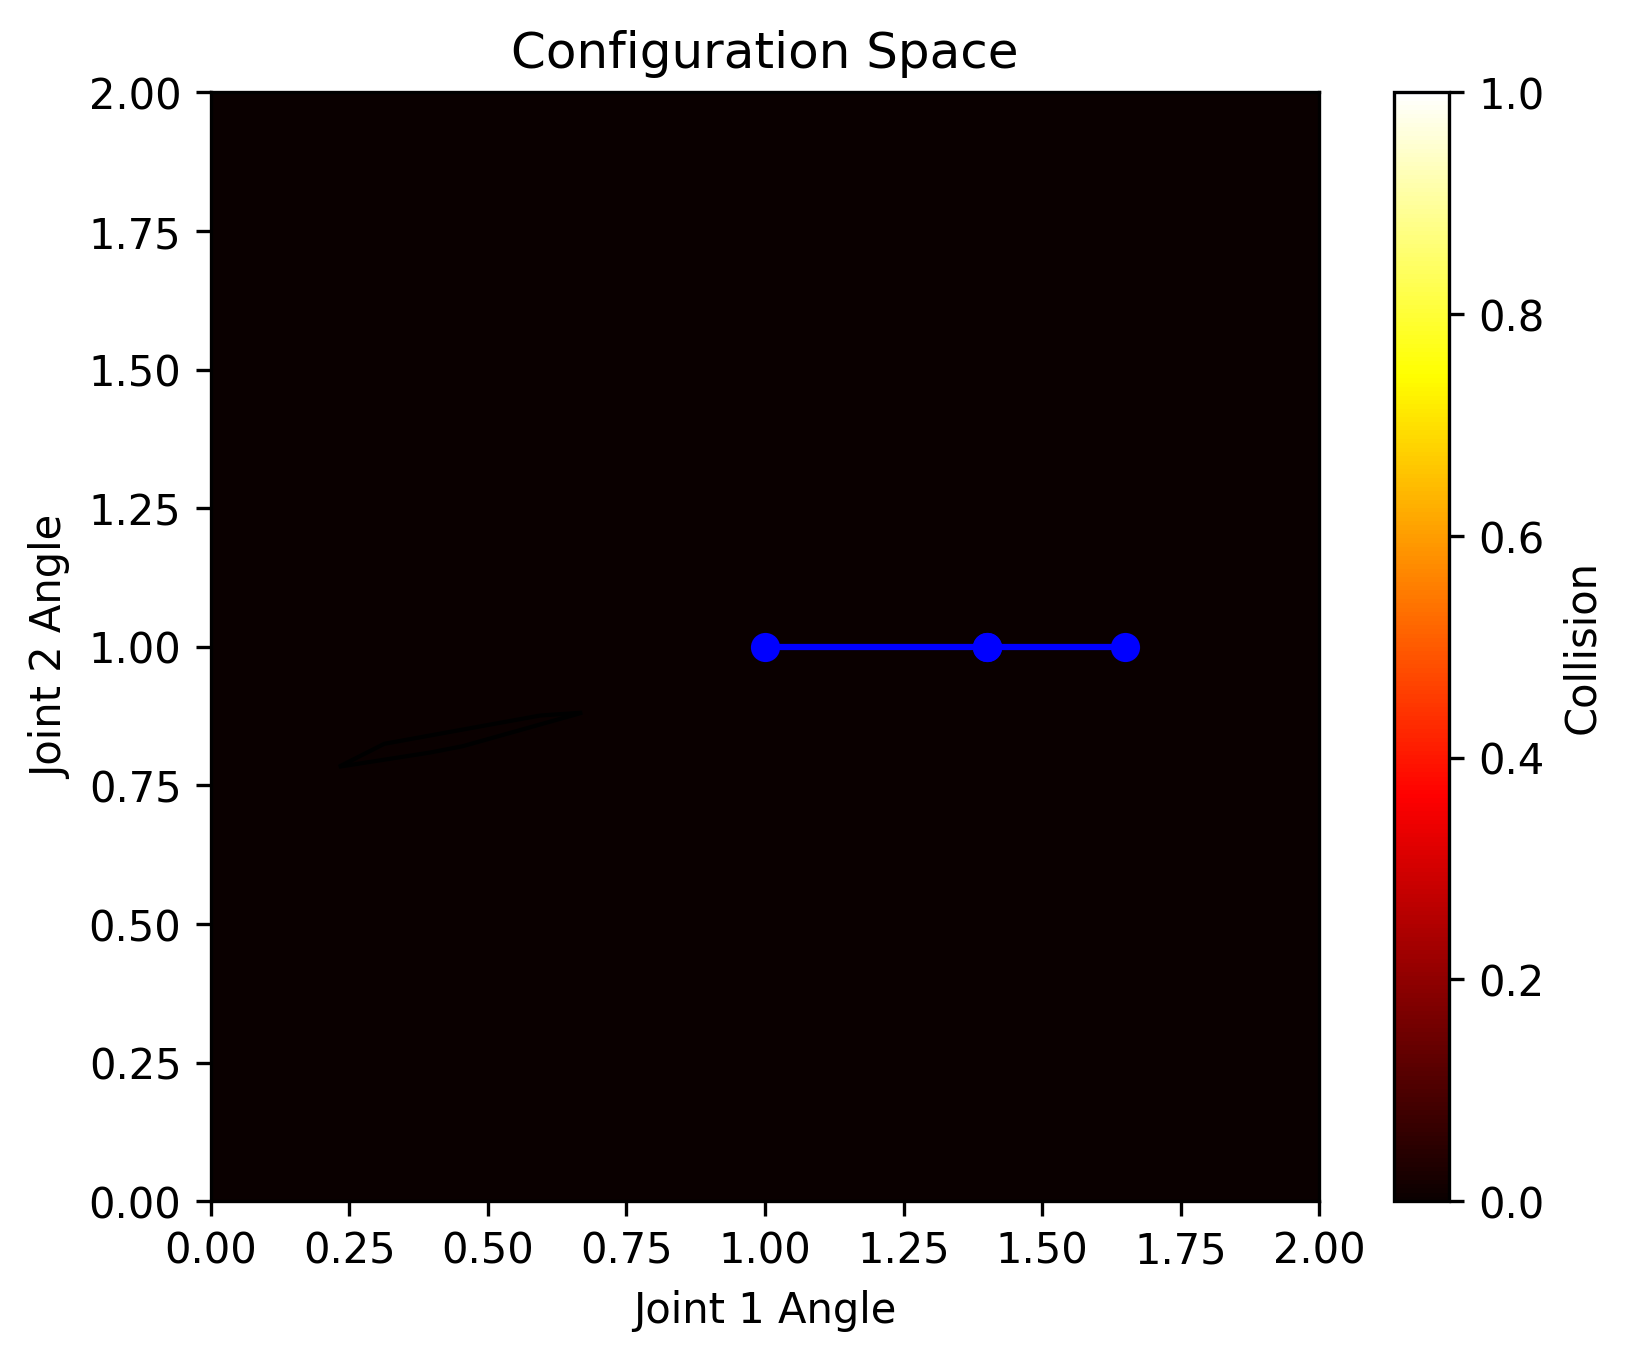
\includegraphics[width=\textwidth]{config_space_scene1.png}
        \caption{Scene 1}
    \end{subfigure}
    \hfill
    \begin{subfigure}{0.45\textwidth}
        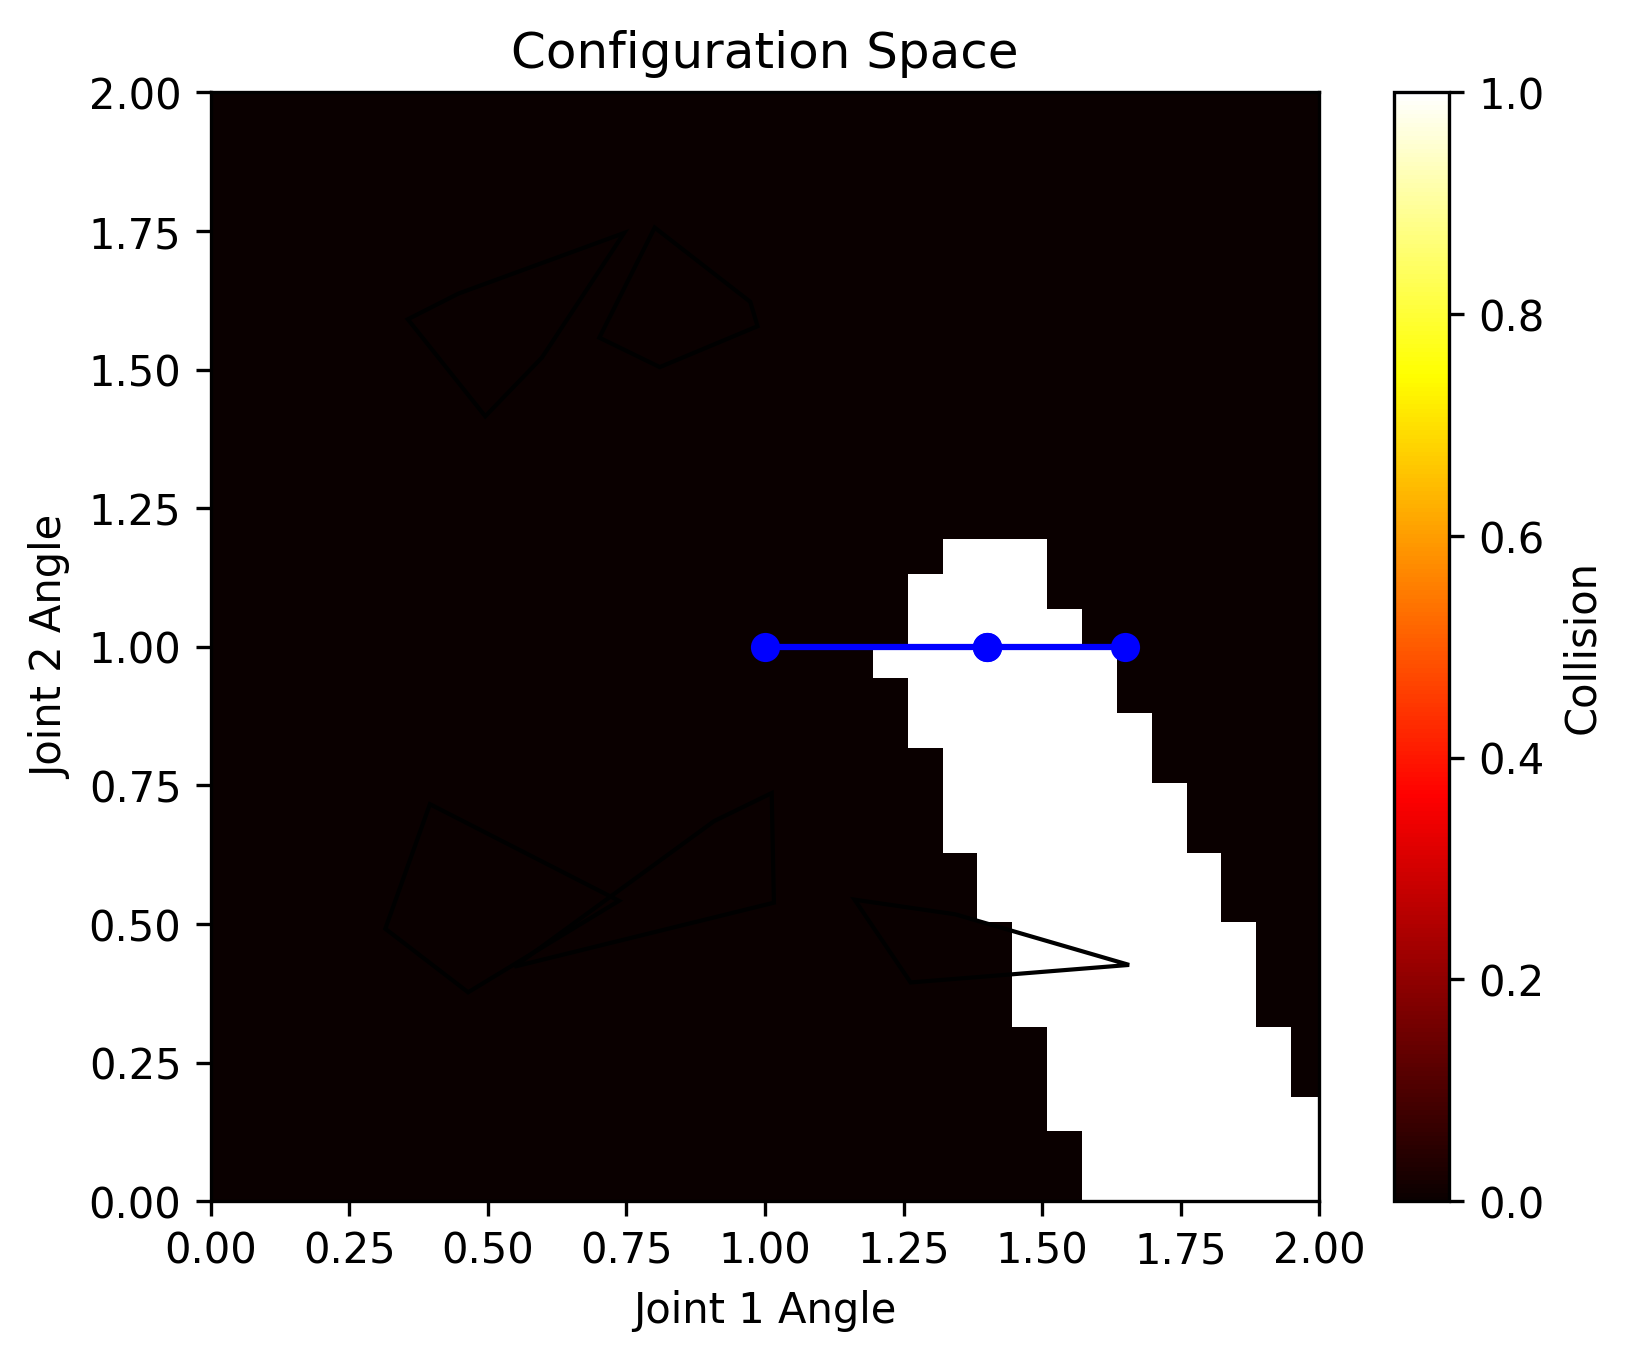
\includegraphics[width=\textwidth]{config_space_scene2.png}
        \caption{Scene 2}
    \end{subfigure}
    \\
    \begin{subfigure}{0.45\textwidth}
        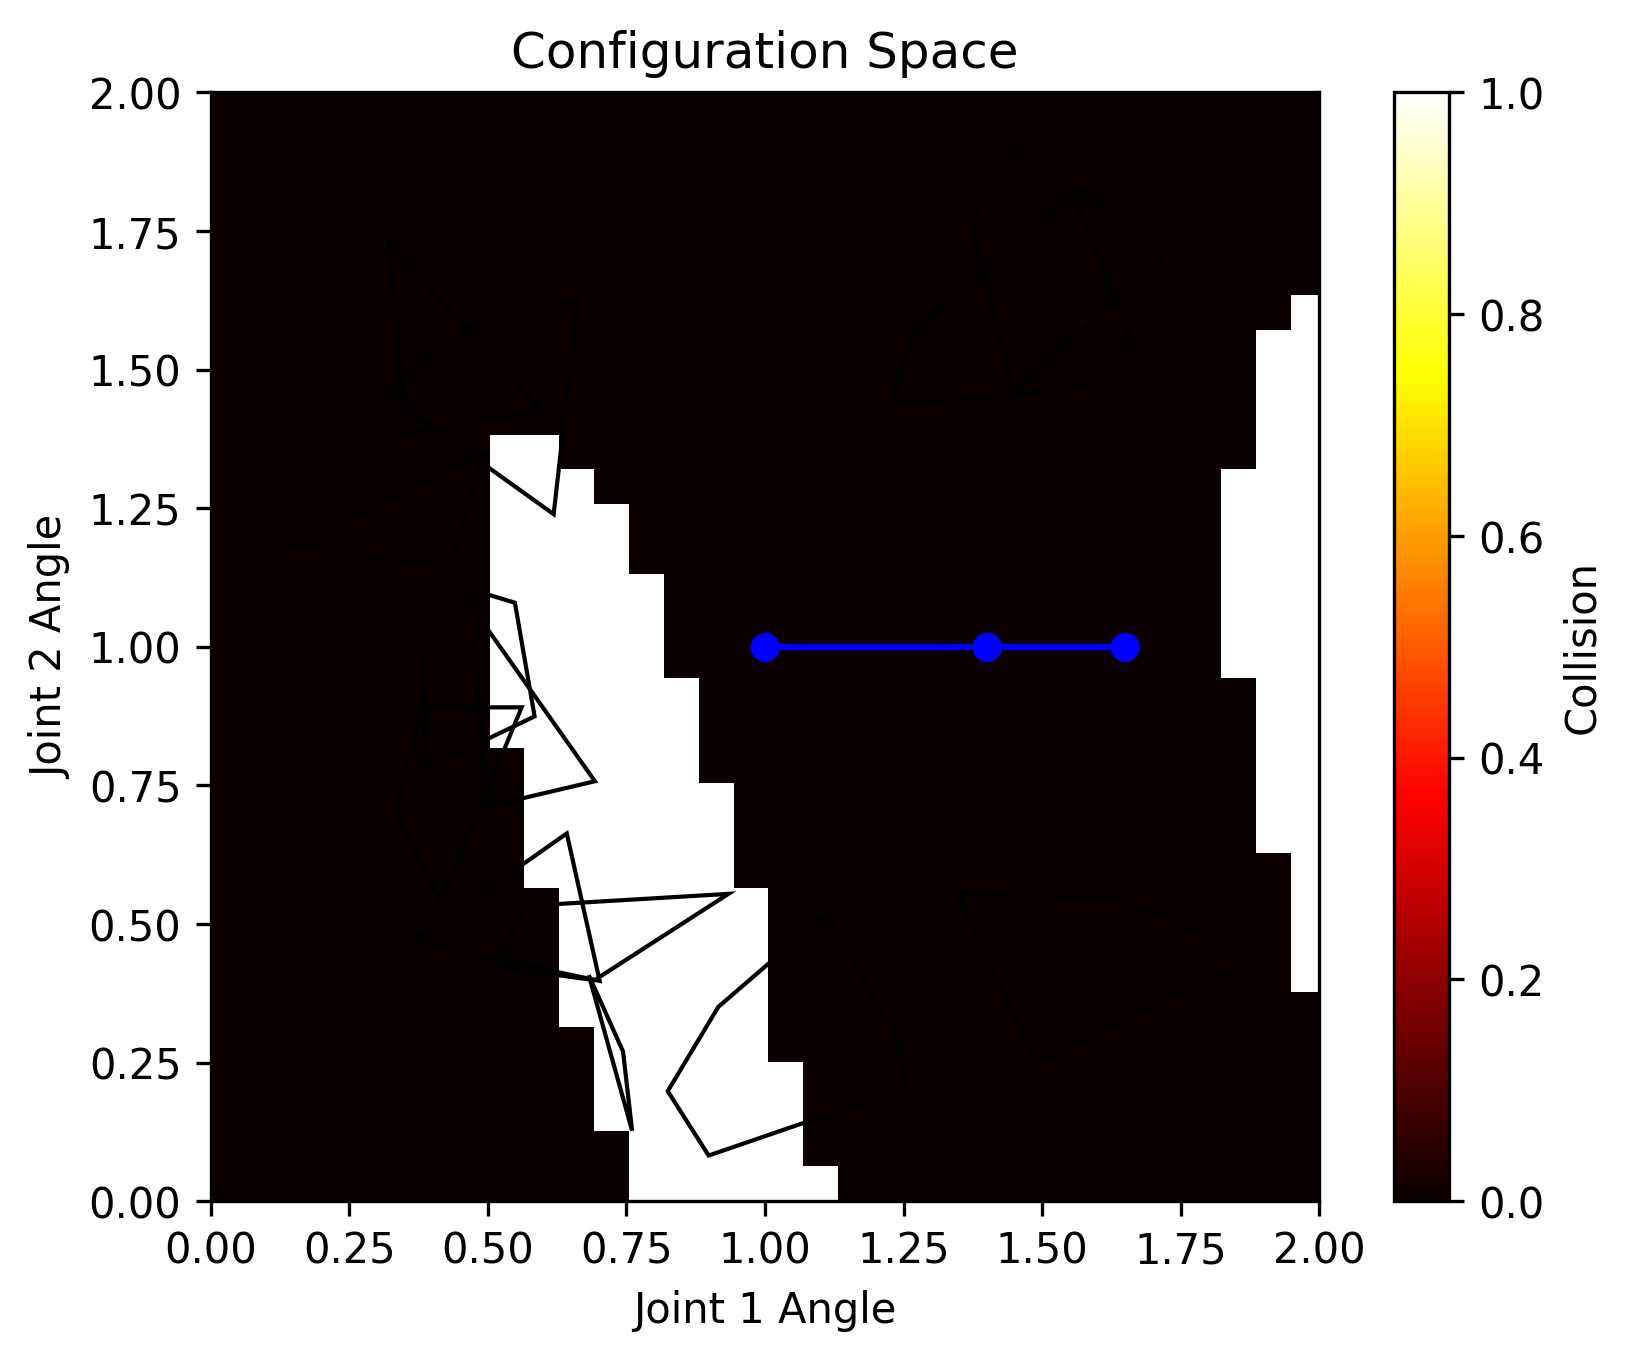
\includegraphics[width=\textwidth]{config_space_scene3.png}
        \caption{Scene 3}
    \end{subfigure}
    \hfill
    \begin{subfigure}{0.45\textwidth}
        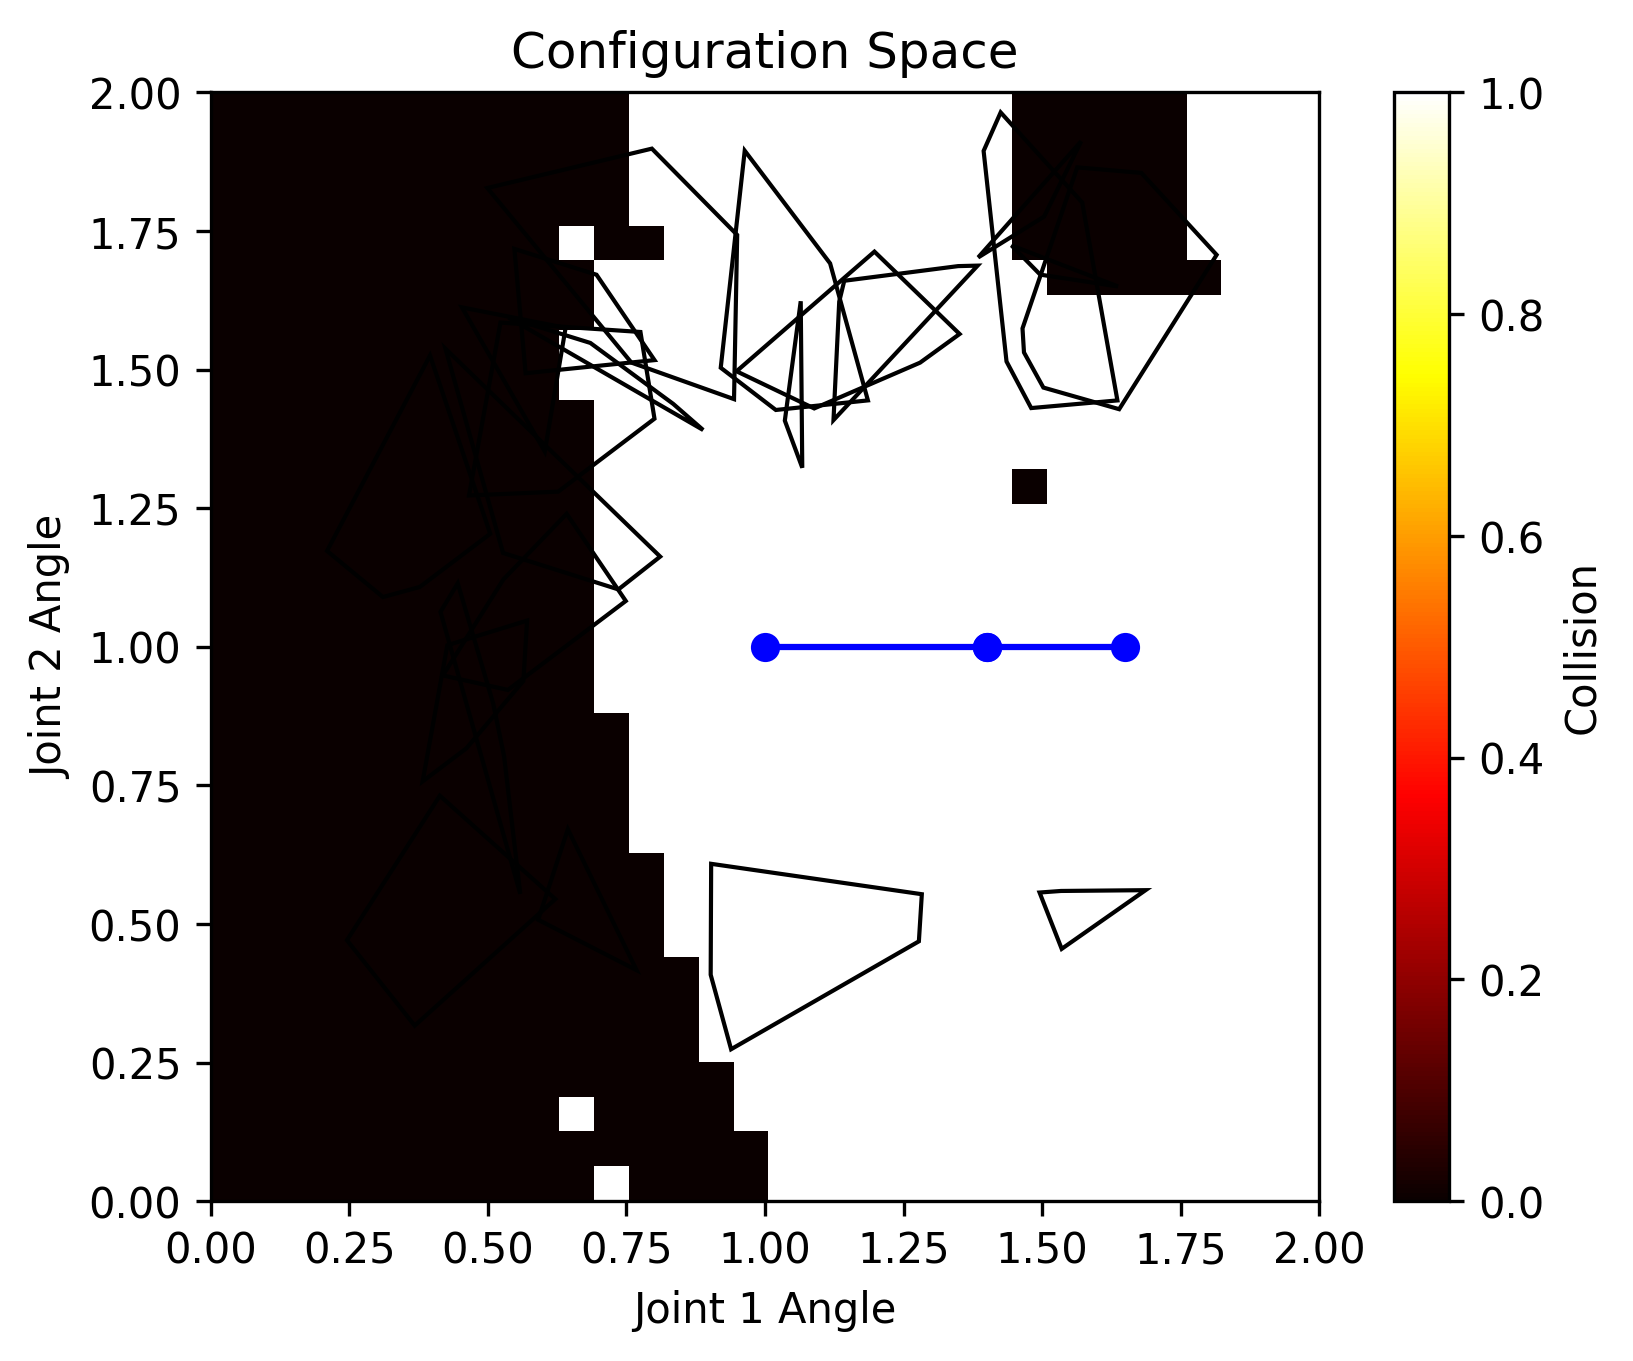
\includegraphics[width=\textwidth]{config_space_scene4.png}
        \caption{Scene 4}
    \end{subfigure}
    \\
    \begin{subfigure}{0.45\textwidth}
        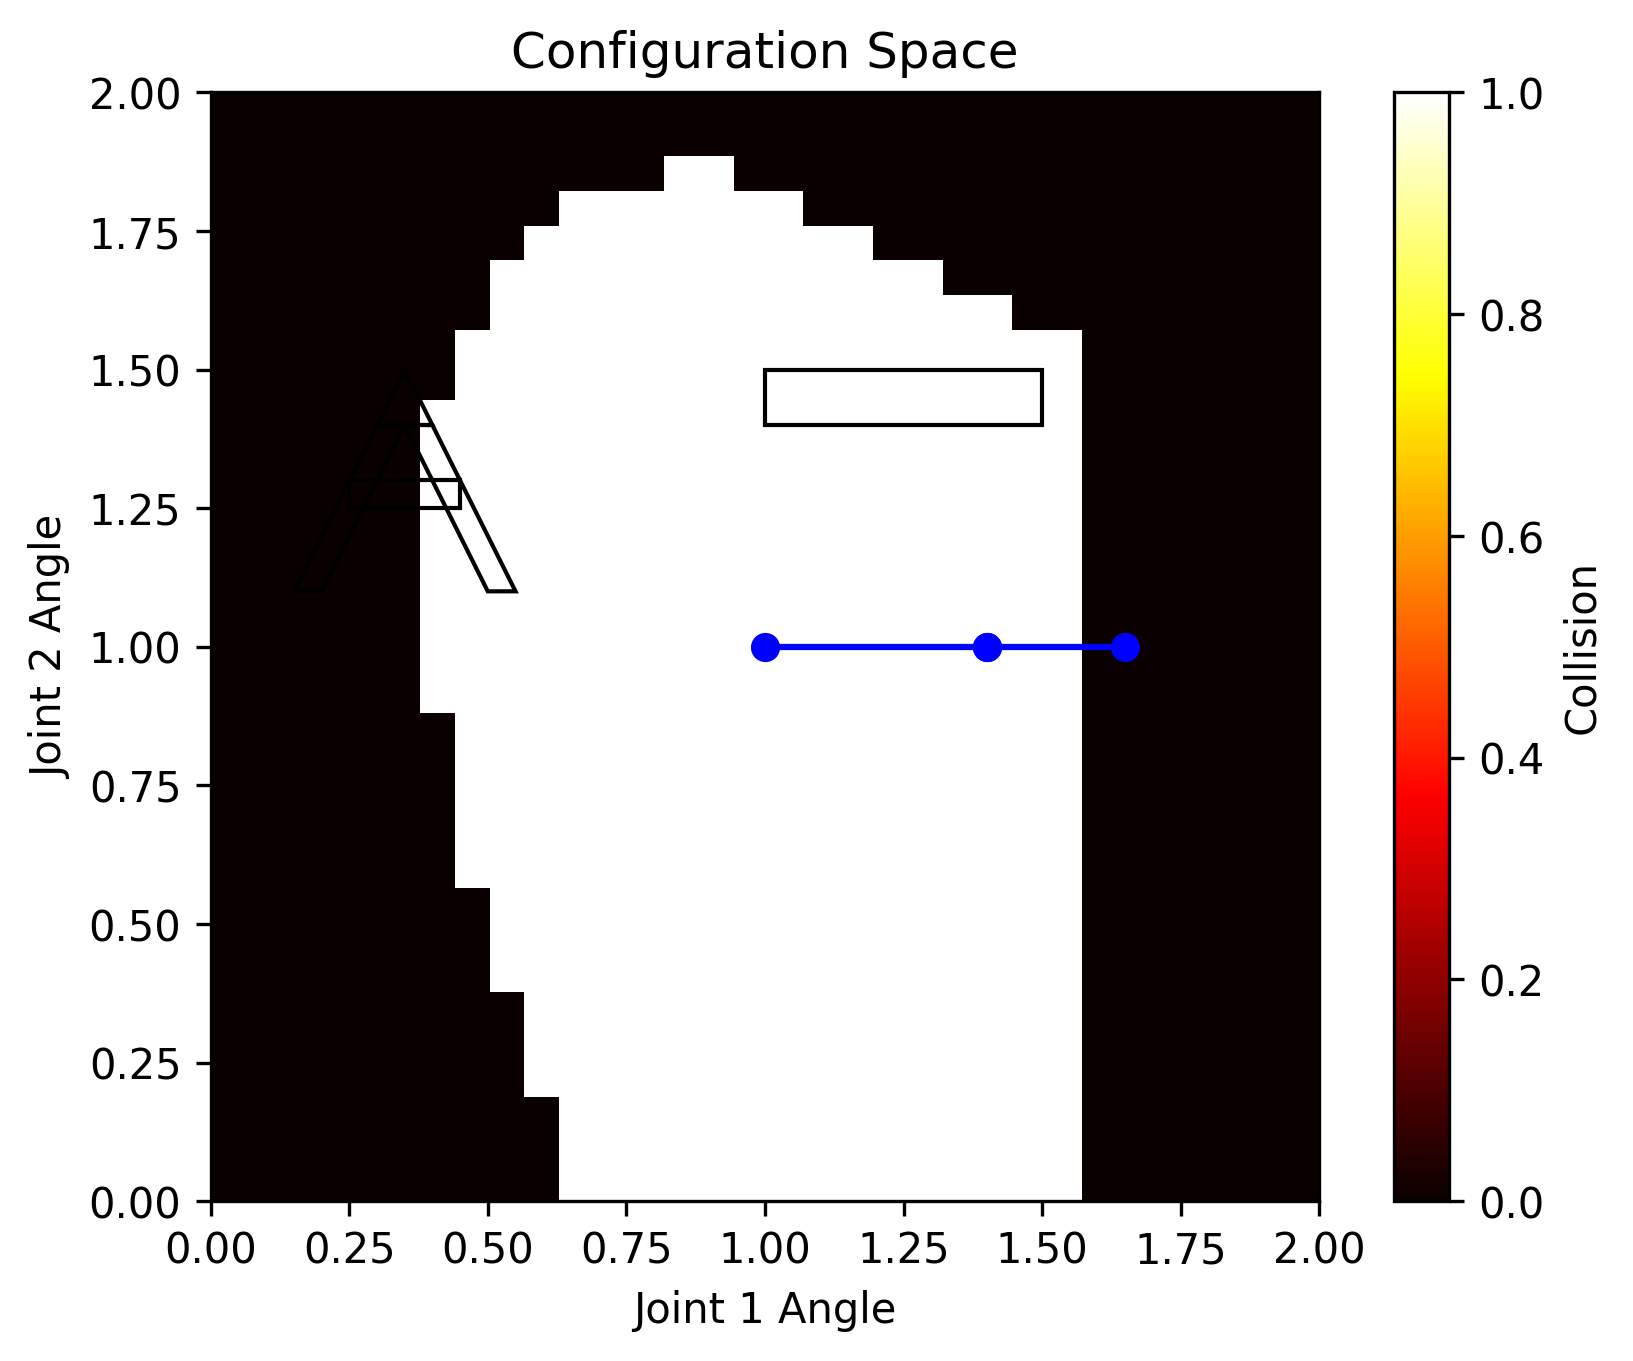
\includegraphics[width=\textwidth]{config_space_scene5.png}
        \caption{Scene 5}
    \end{subfigure}
    \caption{Polygonal scenes with a planar arm, showing different configurations.}
    \label{fig:scenes}
\end{figure}
\end{document}
